\chapter{Модель гистерезисного нейрона} \label{chapter:neuron}

Основой для анализируемой в данной главе модели нейрона послужила монография~\cite{EmelyanovYaroslavsky1990}, в которой рассматривается подход к построению искусственной \acr{NN}, потенциально обладающей рядом интеллектуальных свойств. Особенность работы заключается в том, что автор предлагает оригинальную модель нейрона и показывает через численные и умозрительные эксперименты, что благодаря ряду локальных свойств совокупность нейронов способна демонстрировать нетривиальное поведение. Однако предложенная нейросетевая модель носит ярко выраженный незаконченный характер и кроме того, преследует целью биологическую правдоподобность, что так же отразилось на модели.

Данная диссертационная работа направлена на потенциальную прикладную значимость получаемой \acr{NN}, в частности, при решении задачи контекстно-зависимого распознавания образов. Поэтому предложенный в работе~\cite{EmelyanovYaroslavsky1990} подход был в значительной мере переосмыслен и в результате выработана собственная нейросетевая модель: она не содержит биологически обоснованных переменных и является \socalled \textit{Firing-Rate} моделью~\cite{Dayan2001}, \ie выходным параметром нейрона является усреднённая по времени частота генерации импульсов нейроном (далее, частота), вместо \socalled стохастической \textit{Integrate-And-Fire} модели~\cite{Dayan2001}, в которой моделирование происходит на уровне отдельных импульсов нейрона. Так же присутствует и ряд других изменений, однако полезные в решении нашей задачи идеи были сохранены: использование эффекта гистерезиса и применение совокупности нейронов в виде элементарных логических единиц сети.

%==============================================================================
%                          Формальное определение модели
%==============================================================================
\section{Формальное определение} \label{section:neuron_model}

Формальная модель нейрона выглядит следующим образом:
\begin{equation}
	\label{eq:single_neuron_model}
    \begin{cases}
	    d\scalar{u}/d\scalar{t} &= \vector{x}^\top \vector{w} - \scalar{p} - \mu \scalar{u}, \\
        \scalar{\nu}            &= f\left( \scalar{u}, \theta \right), \\
    \end{cases}
\end{equation}
где $\scalar{u} \in \specialset{R}$ --- потенциал нейрона, $\vector{x} \in \specialset{R}^{N}$ -- входной вектор нейрона (входной сигнал), $\vector{w} \in \specialset{R}^{N}$ --- вектор весовых коэффициентов связей нейрона,  $\scalar{p}$ --- внутренний порог нейрона, $\mu$ --- константа, характеризующая скорость убывания потенциала нейрона, $\scalar{\nu} \in \left[0;1\right]$ --- частота нейрона (выходной сигнал), $\theta$ --- управляющий параметр сети, функциональный смысл которого будет рассмотрен в следующих главах.

Функция активации $f: \specialset{R} \to \left[0;1\right]$ отражает нелинейное преобразование потенциала нейрона $\scalar{u}$ в его выходную частоту $\scalar{\nu}$. В данной главе будут рассмотрены две функции активации, изображённые \onfigure~\ref{img:model_activation_functions}:
\begin{itemize}
	\item оригинальная функция $s$, полученная на основе функции динамического порога нейрона $\text{П}^\text{Д}$ из работы~\cite{EmelyanovYaroslavsky1990}, но отличающаяся от неё, т.к. функция $\text{П}^\text{Д}$ отражает работу на уровне отдельный импульсов и кроме того, она не была задана автором аналитически:
		\begin{equation}
			s(\scalar{u}, \theta) = 
		\end{equation}
	\item широко распространённая в области машинного обучения сигмоидальная функция $\sigma$:
		\begin{equation}
			\sigma(\scalar{u}, \theta) = 
		\end{equation}
\end{itemize}

%Функция $s$ была получена на основе функции динамического порога нейрона из работы~\cite{EmelyanovYaroslavsky1990} (), но отличается от неё: во-первых, 

\begin{figure}[ht]
    \makebox[\textwidth][c]{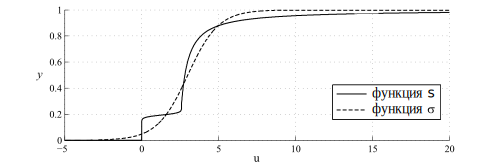
\includegraphics[width=1.0\textwidth]{model_activation_functions}}
    \caption{Вид функции активации: а) \inquotes{оригинальной} функции $s(u)$; б) сигмоидальной функции $\sigma(s)$.}
    \label{img:model_activation_functions}
\end{figure}

\begin{figure}[ht]
	\makebox[\textwidth][c]{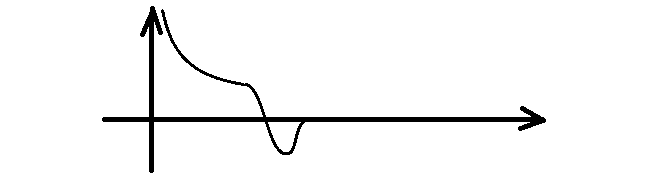
\includegraphics[width=1.0\textwidth]{model_extern_dynamic_threshold}}
	\caption{Вид функции динамического порога нейрона $\text{П}^\text{Д}$ из работы~\cite{EmelyanovYaroslavsky1990}. \todo{В приложение?..}}
	\label{img:model_extern_dynamic_threshold}
\end{figure}

%==============================================================================
%                       Анализ точек равновесия модели
%==============================================================================
\section{Анализ точек равновесия} \label{section:neuron_equilibrium}

%==============================================================================
%                       Бифуркационный анализ модели
%==============================================================================
\section{Бифуркационный анализ} \label{section:neuron_bifurcation}

%==============================================================================
%                       Характерные параметры модели
%==============================================================================
\section{Характерные свойства} \label{section:neuron_parameters}

%==============================================================================
%                       Характерная динамика модели
%==============================================================================
\section{Характерная динамика} \label{section:neuron_dynamic}

%==============================================================================
%               Моделирование нейросетевого конечного автомата
%==============================================================================
\section{Моделирование нейросетевого конечного автомата} \label{section:neuron_fsm}

\todo{Вводная часть...}

\subsection{Построение модели конечного автомата}

Определим детерминированный конечный автомат (\acr{FSM})~\cite{Hopcroft2008} как формальную математическую структуру $M = \left( \usualset{A}, \usualset{S}, s_{0}, \delta \right)$, где $\usualset{A}$ --- конечное множество входных символов (входной алфавит), $\usualset{S}$ --- конечное множество состояний автомата, $s_{0} \in \usualset{S}$ --- начальное состояние автомата, $\delta\!: \usualset{S}\!\times\!\usualset{A} \to \usualset{S}$ --- функция перехода, отображающая упорядоченную пару элементов (состояние автомата и входной символ) в новое состояние автомата. Если мы обозначим через $q \in \usualset{S}$ текущее состояние автомата, которое в начальный момент времени совпадает с $s_{0}$, то функционирование автомата заключается в последовательном считывании символов $a_{i}$ из входной последовательности $\left\{ a_{0} a_{1} \ldots | a_{j} \in \usualset{A} \right\}$ и переходе в новое состояние: $q = \delta \left( q, a_{i} \right)$. Стоит отметить, что в структуру $M$ часто добавляют множество \socalled заключительных состояний $\usualset{F} \subseteq \usualset{S}$ для верификации считанной входной последовательности, однако в данной работе в этом нет необходимости.

Построение нейросетевой модели по заданной структуре \acr{FSM} можно разбить на две части: построение топологии сети и подбор весовых коэффициентов связей сети. Для задания топологии в первую очередь необходимо каждому элементу всех множеств структуры $M$ поставить в соответствие свой нейрон $n_{i}$: обозначим множество $\left\{ n_{k} | k = \usualset{A} \right\}$, соответствующее множеству $\usualset{A}$, как множество \inquotes{входных} нейронов, множество $\left\{ n_{k} | k = \usualset{S} \right\}$, соответствующее множеству $\usualset{S}$, как множество нейронов \inquotes{состояний} и множество $\left\{ n_{k} | k = D(\delta) \right\}$, соответствующее множеству $S\!\times\!A$ (исключая элементы, для которых отображение $\delta$ не определено), как множество нейронов \inquotes{переходов}. Таким образом, сеть будет состоять из $N = \left|\usualset{A}\right| + \left|\usualset{S}\right| + \left|D(\delta)\right|$ нейронов.

Далее каждому переходу, заданному как элемент множества $\{ \left( s_{i}, s_{j}, a_{k} \right) | \exists \delta\!: s_{i}\!\times\!a_{k} \to s_{j} \}$, необходимо поставить в соответствие набор связей между нейронами сети. Учтём, что в любой момент времени может считываться только один входной символ и должен быть активен только один нейрон \inquotes{состояния} (исключая периоды смены текущего состояния \acr{FSM}, которые связаны с инертностью системы). Поэтому переход из одного состояния в другое является результатом взаимодействия тех нейронов, которые непосредственно соответствуют данному переходому в структуре $M$, а активность остальных должна быть пренебрежимо мала. В результате такой локализации вычислений нейронные связи в сети можно представить в виде типизированного набора, соответствующего каждому переходу в \acr{FSM}: $\beta_{st}$ --- двунаправленная тормозная связь между $n_{s_{i}}$ и $n_{s_{j}}$, $\beta_{tr}$ --- тормозная связь от $n_{s_{i}\!\times\!a_{k}}$ к $n_{a_{k}}$, $\gamma_{st}$ --- возбуждающая связь от $n_{s_{i}}$ к $n_{s_{i}\!\times\!a_{k}}$, $\gamma_{tr}$ -- возбуждающая связь от $n_{s_{i}\!\times\!a_{k}}$ к $n_{s_{j}}$, $\gamma_{in}$ --- возбуждающая связь от $n_{a_{k}}$ к $n_{s_{i}\!\times\!a_{k}}$. \todo{Таким образом, матрица связей \acr{NN} будет имеет следующий вид: ...}

Значения весовых коэффициентов связей подбираются путём решения системы неравенст, описывающей требуемое от элементов сети поведение. Для произвольного перехода $s_{i}\!\times\!a_{k}~\to~s_{j}$ эти требования можно сформулировать следующим образом:. \todo{Формально это соответствует следующей системе уравнений:}

Данная схема позволяет построить для произволного \acr{FSM} функционально эквивалентную нейросетевую модель. Перед началом моделирования начальное состоние $S_{0}$ может быть задано явно, например, как одно из начальных условий: $\nu_{s_{0}} = \nu^{high}$.

Для наглядности \onfigure~\ref{img:fsm_example_topology}а изображена простейшая схема \acr{FSM} с $\usualset{A} = \{ a_{1}, a_{2} \}$, $\usualset{S} = \{ s_{1}, s_{2}, s_{3} \}$ и функцией $\delta$, определённой как $\{ s_{1}\!\times\!a_{1} \to s_{2}$, $s_{2}\!\times\!a_{1} \to s_{3}$, $s_{3}\!\times\!a_{2} \to s_{1} \}$. Результат применения описанного выше преобразования --- функционально эквивалентная \acr{NN}, изображённая \onfigure~\ref{img:fsm_example_topology}б (на рисунке также изображены рекуррентные связи нейронов $\alpha_{st}$ и $\alpha_{tr}$). Используя параметры сети \todo{параметры}, можно вычислить коэффициенты связей (\seefigure~\ref{img:fsm_example_weights}): \todo{коэффициенты}.

\begin{figure}[ht]
    \makebox[\textwidth][c]{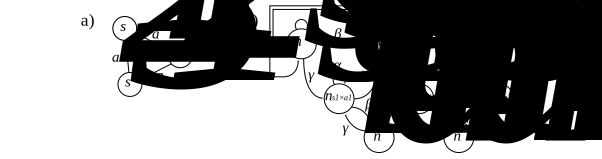
\includegraphics[width=1.0\textwidth]{fsm_example_topology}}
    \caption{Пример построения нейросетевого \acr{FSM}: а) диаграмма состояний автомата; б) эквивалентная диаграмме состояний схема \acr{NN}.} 
    \label{img:fsm_example_topology}  
\end{figure}

\begin{figure}[ht]
    \makebox[\textwidth][c]{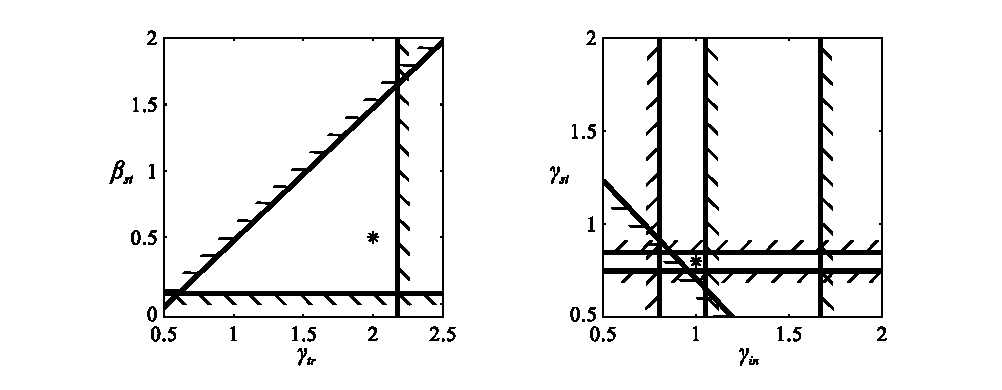
\includegraphics[width=1.2\textwidth]{fsm_example_weights}}
    \caption{Допустимые области значений для весовых коэффициентов, полученные при использовании параметров: \todo{значения параметров}. Ограничения обусловлены функциональными требованиями, наложенными на различные типы нейронов. } 
    \label{img:fsm_example_weights}  
\end{figure}


\subsection{Результаты численного моделирования}

Результат моделирования простейшей схемы \acr{FSM} из предыдущего подраздела (\seefigure~\ref{img:fsm_example_topology}) представлен \onfigure~\ref{img:fsm_example_dynamic}, на котором отражена частота нейронов \inquotes{состояний} и периоды предъявления входных символов. Видно, что при подаче допустимых входных символов, \ie для которых определён переход из текущего состояния, происходит смена конфигурации: соответствующий текущему состоянию нейрон становится неактивным, а соответствующий новому состоянию --- активным. В то же время, при подаче недопустимого символа (интервал времени $[350; 375]$) состояние сети качественно остаётся без изменений. Кроме того, стоит отметить что непрерывное предъявление входного символа приводит к последовательной смене состояний до тех пор, пока схема автомата это допускает (интервал времени $[450; 500]$), что отражает периодичность происходящих в модели процессов.

\begin{figure}[ht]
    \makebox[\textwidth][c]{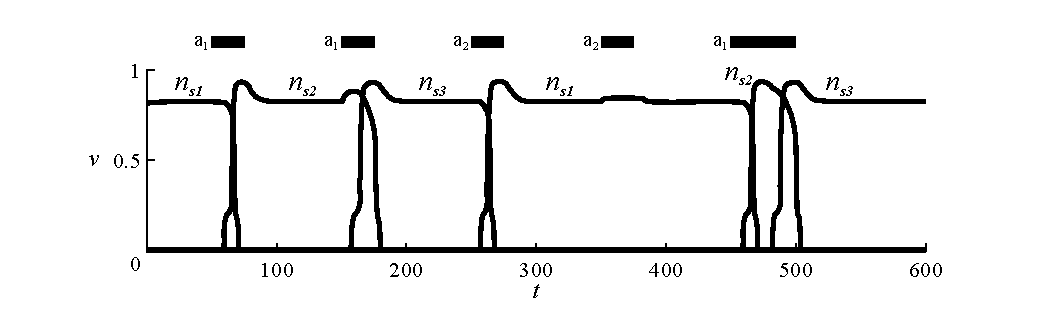
\includegraphics[width=1.1\textwidth]{fsm_example_dynamic}}
    \caption{Динамика нейронов \inquotes{состояний} нейросетевой модели \acr{FSM}, представленной \onfigure~\ref{img:fsm_example_topology}б. Верхние горизонтальные линии отражают временн\'{ы}е периоды считывания входных символов.} 
    \label{img:fsm_example_dynamic}  
\end{figure}

Также работоспособность данного подхода проверялась и на более сложных примерах \acr{FSM}, один из которых приведён \onfigure~\ref{img:fsm_model_topology}, --- стоит отметить наличие в диаграмме состояний циклов и двойных переходов (наличие двойных дуг от одного состояния к другому). Как и ранее, в результате применения описанного выше преобразования была получена функционально эквивалентная нейросетевая модель со следующими параметрами: \todo{параметры}. Различные численные эксперименты, один из которых приведён \onfigure~\ref{img:fsm_model_dynamic}, показали, что нейросетевая модель автомата успешно обрабатывает любую последовательность входных символов, игнорируя недопустимые символы. При этом работоспособность сохраняется и при обработке достаточно длинных последовательностей (максимальная использованная длина последовательности составила 1000 символов) и при наличии больших временн\'{ы}х задержек между предъявлениями символов (максимальная использованная задержка составила порядка 10000 единиц), что подтверждает работоспособность данного подхода.

\begin{figure}[ht]
    \makebox[\textwidth][c]{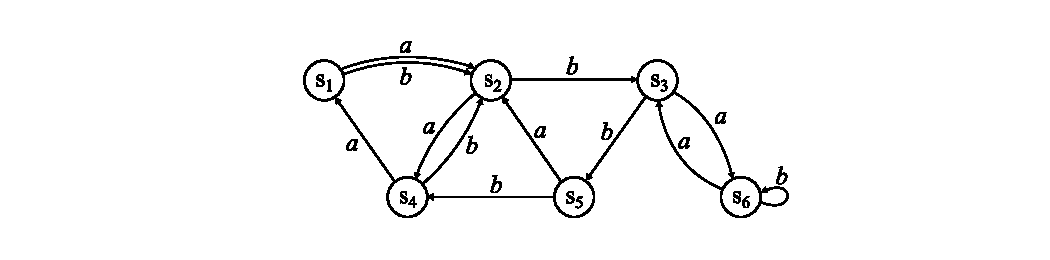
\includegraphics[width=1.2\textwidth]{fsm_model_topology}}
    \caption{Диаграмма состояний \acr{FSM}, использованного в процессе моделирования.}
    \label{img:fsm_model_topology}  
\end{figure}

\begin{figure}[ht]
    \makebox[\textwidth][c]{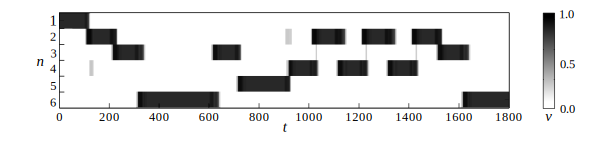
\includegraphics[width=1.1\textwidth]{fsm_model_dynamic}}
    \caption{Результаты численного моделирования нейросетевого \acr{FSM}, представленного \onfigure~\ref{img:fsm_model_topology}. Ось ординат соответствует индексам нейронов \inquotes{состояний}. Значение частоты нейронов выражено оттенками серого в соответствии со шкалой справа.} 
    \label{img:fsm_model_dynamic}  
\end{figure}

%==============================================================================
%                               Выводы по главе
%==============================================================================
\section{Выводы по главе \thechapter} \label{section:neuron_concls}



